\documentclass[10pt, a4paper,spanish]{article}

\usepackage[utf8]{inputenc}
\usepackage[spanish]{babel}

\usepackage[T1]{fontenc}

\usepackage[hmarginratio=1:1,top=32mm,columnsep=20pt]{geometry}
\usepackage[hang, small,labelfont=bf,up,textfont=it,up]{caption}

\usepackage{float}

\usepackage{amsmath}

\usepackage{enumitem}

\usepackage{graphicx}
\graphicspath{ {images/} }


\usepackage{titlesec}
\renewcommand\thesection{\Roman{section}}
\renewcommand\thesubsection{\Roman{subsection}}
\titleformat{\section}[block]{\large\scshape\centering}{\thesection.}{1em}{}
\titleformat{\subsection}[block]{\large}{\thesubsection.}{1em}{}

\usepackage{fancyhdr}
\pagestyle{fancy}
\fancyhead{}
\fancyfoot{}
\fancyhead[C]{ \today \ $\bullet$ Ingeniería del Conocimiento $\bullet$ Clips 2}
\fancyfoot[RO]{\thepage}

%-------------------------------------------------------------------------------
%	TITLE SECTION
%-------------------------------------------------------------------------------

\title{\vspace{-15mm}\fontsize{24pt}{10pt}\selectfont\textbf{Clips 2}} % Article title

\author{
	Fernández Angulo, Óscar \\
	\and
	García Prado, Sergio
}

\date{\today}

%-------------------------------------------------------------------------------

\begin{document}

	\maketitle % Insert title

	\thispagestyle{fancy} % All pages have headers and footers


%-------------------------------------------------------------------------------
%	TEXT
%-------------------------------------------------------------------------------

	\section{Sistema Cardiovascular Humano}

		\begin{figure}[H]
			\begin{center}
				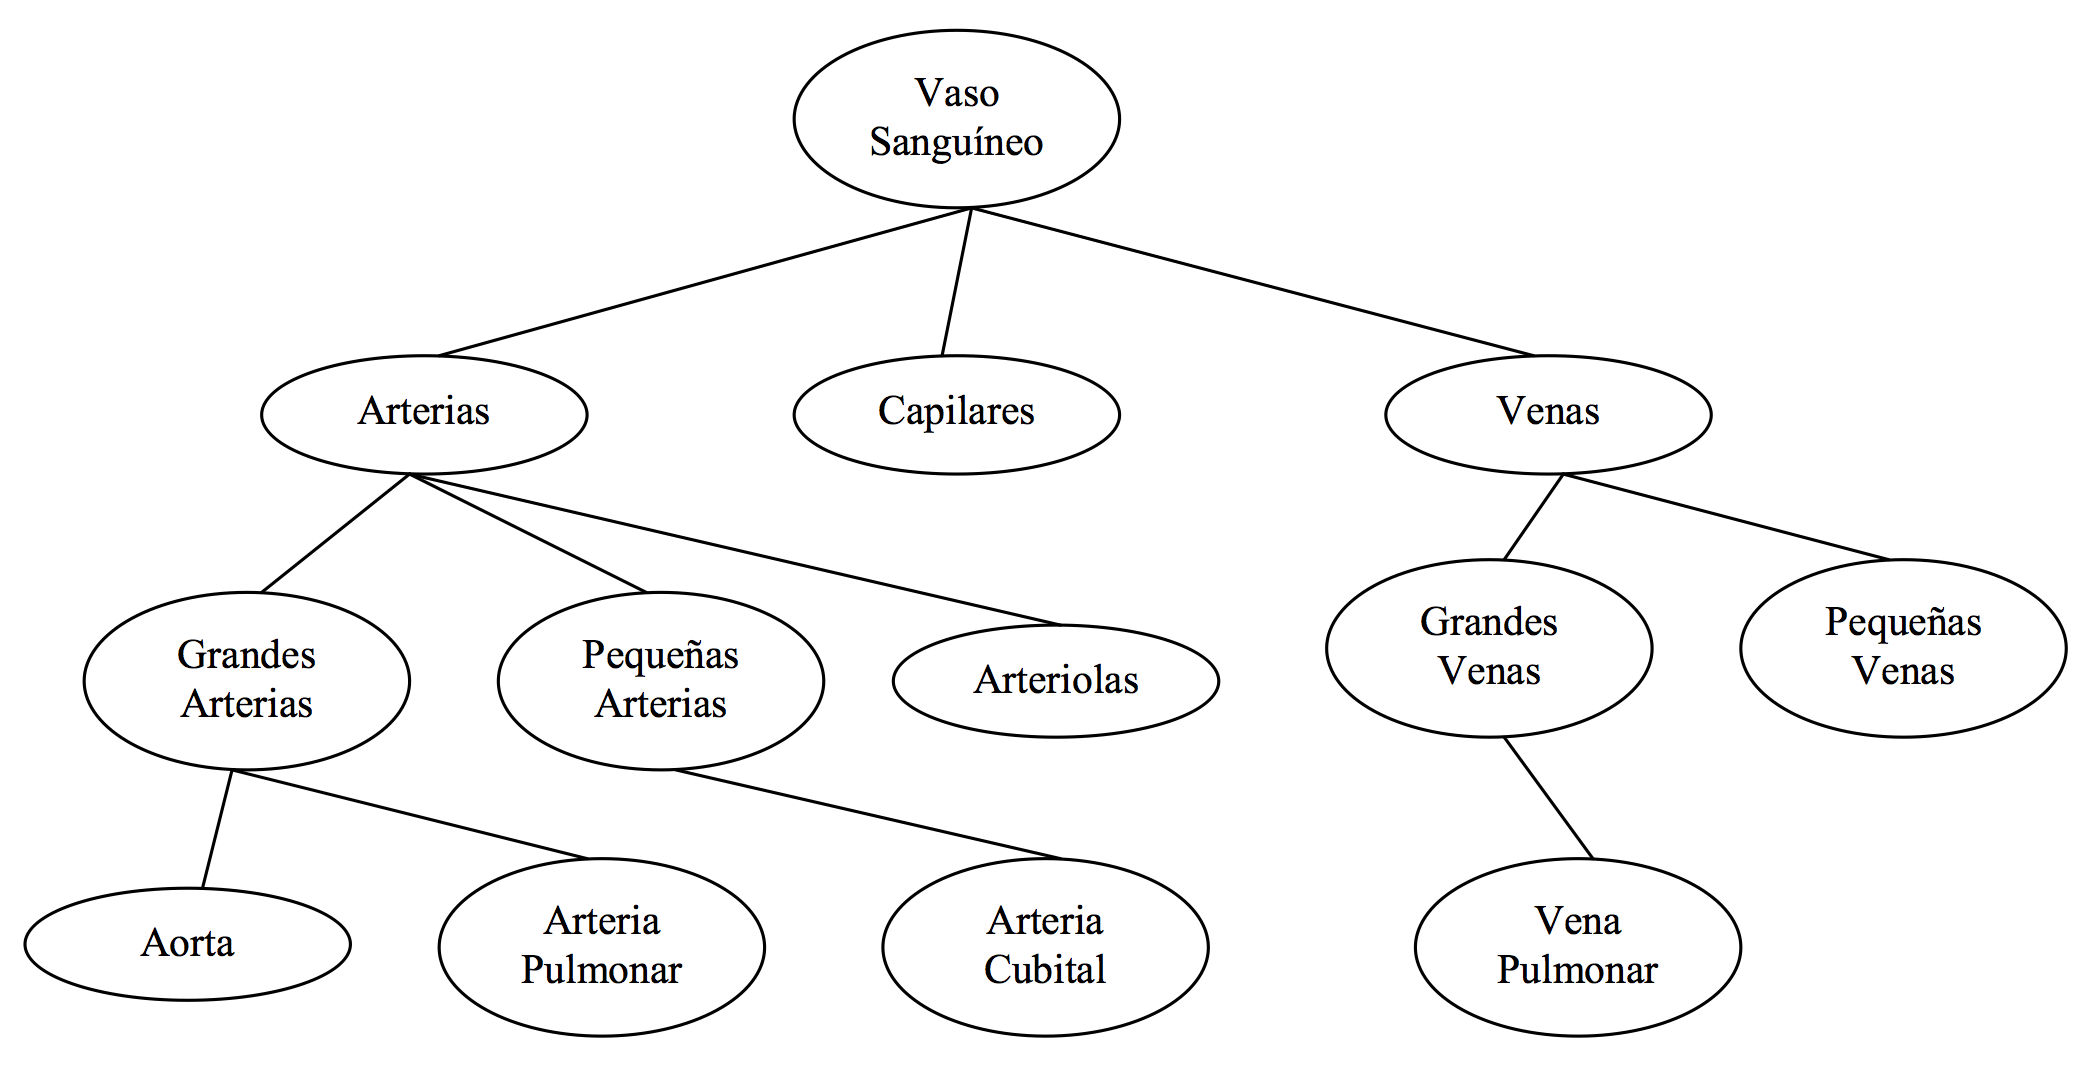
\includegraphics[width=0.75\textwidth]{diagram}
			\end{center}
		\end{figure}

		\begin{enumerate}
			\item El sistema cardiovascular está formado por el corazón y una red de vasos sanguíneos interconectados.

			\item Los vasos sanguíneos se subdividen en tres categorías: arterias, capilares y venas.

			\item Estas categorías se subdividen como indica la figura.

			\item La aorta, la arteria y venas pulmonares y la arteria cubital son ejemplos de vasossanguíneos específicos

			\item Las arterias transportan sangre desde el corazón hasta los capilares de los tejidos y sedistinguen de otros vasos por poseer una pared gruesa formada por capas de células musculares. En la mayoría de los casos, las arterias transportan sangre con un elevado contenido de oxigeno.

			\item Contrariamente a las arterias, las venas transportan sangre desde los capilares de los tejidos al corazón. Tienen una pared relativamente delgada que contiene menos células musculares que las de las arterias, pero más tejido fibroso. Usualmente, las venas contienen sangre pobre en oxigeno.

			\item La presión sanguínea media en las arterias es relativamente elevada (40-100 mmHg), frente a una presión media inferior a 10 mmHg en la mayoría de las venas.

			\item Las arterias pulmonares son un ejemplo de excepción a la descripción anterior. Estas arterias transfieren sangre del corazón a los pulmones y poseen una gruesa pared muscular. Por ello se las considera arterias. Sin embargo, estas arterias transfieren sangre con bajo contenido en oxigeno y su presión media es más bien baja (13 mmHg).

			\item La presión sanguínea media de un paciente se calcula a partir de los valores de la presión sanguínea muestreados en un intervalo de tiempo. La presión sanguínea oscila entre un valor máximo, denominado presión sistólica, y un nivel mínimo denominado presión diastólica; la diferencia entre ambas se denomina presión del pulso. En la práctica diaria, en vez de calcular la presión sanguínea media, solo suelen registrarse los valores de las presiones sistólica y diastólica.

			\item La tabla 1 muestra la presión sanguínea media, el diámetro y el porcentaje total de volumen de sangre para cada categoría.

			\item El funcionamiento del sistema cardiovascular suele explicarse recurriendo a la analogía con un sistema hidráulico. Este sistema hidráulico estaría compuesto por una bomba (corazón), un conjunto de conducciones interconectadas (vasos sanguíneos) y un contenedor conectado a la bomba (presurizador) lleno de agua (sangre).

			\item La información presentada en esta discusión es generalmente aplicable a un adulto sano. Por ejemplo, si un paciente sufre una estenosis (estrechamiento) arterial, la presión sanguínea distal (en dirección opuesta al corazón) en la estenosis de la arteria es próxima a cero.

			\item Cualquier desarreglo que afecta al corazón o a los vasos sanguíneos se considera una enfermedad cardiovascular. Así, un aneurisma (protuberancia) de la arteria abdominal, una estenosis arterial o la arteriosclerosis, que afectan a los vasos sanguíneos, son enfermedades cardiovasculares. La regurgitación aórtica, que ocurre cuando las válvulas de las aortas no son totalmente estancas, es una enfermedad cardiovascular que afecta al corazón.

			\item Para realizar la diagnosis médica, se puede recurrir a una descripción detallada de la estructura y funcionamiento del sistema cardiovascular (conocimiento “profundo” o detallado) o se puede recurrir a las asociaciones típicas y bien documentadas entre síntomas (quejas del paciente), evidencia clínica (resultado de test o pruebas realizadas por equipos médicos), causas y enfermedades (conocimiento superficial, de naturaleza heurística). Aunque esta distinción entre conocimiento detallado y superficial no siempre es clara y precisa, en la práctica diaria de la profesión el conocimiento superficial juega un papel importante.

			\item Así, cuando un paciente se queja de un dolor abdominal, una auscultación permite percibir un rumor abdominal y al palpar el abdomen del paciente se siente una masa pulsante, un aneurisma de la arteria abdominal probablemente cause estos síntomas y evidencias clínicas.

			\item Si la presión sistólica del paciente supera los 140 mmHg, la presión del pulso es superior a 50 mmHg, y al auscultar al paciente se percibe un rumor sistólico o una dilatación del corazón, todo ello puede estar causado por una regurgitación aórtica.

			\item Como último ejemplo, si un paciente siente calambres en las piernas al andar, que desaparecen tras uno o dos minutos de descanso, la presencia de una estenosis en una de las arterias de las piernas es más que probable. A su vez, la estenosis suele deberse a un problema de arteriosclerosis, especialmente si el paciente pertenece a algún grupo de riesgo: obeso o fumador durante más de 15 años o edad superior a 50 años.

		\end{enumerate}

		\begin{figure}[H]
			\begin{center}
				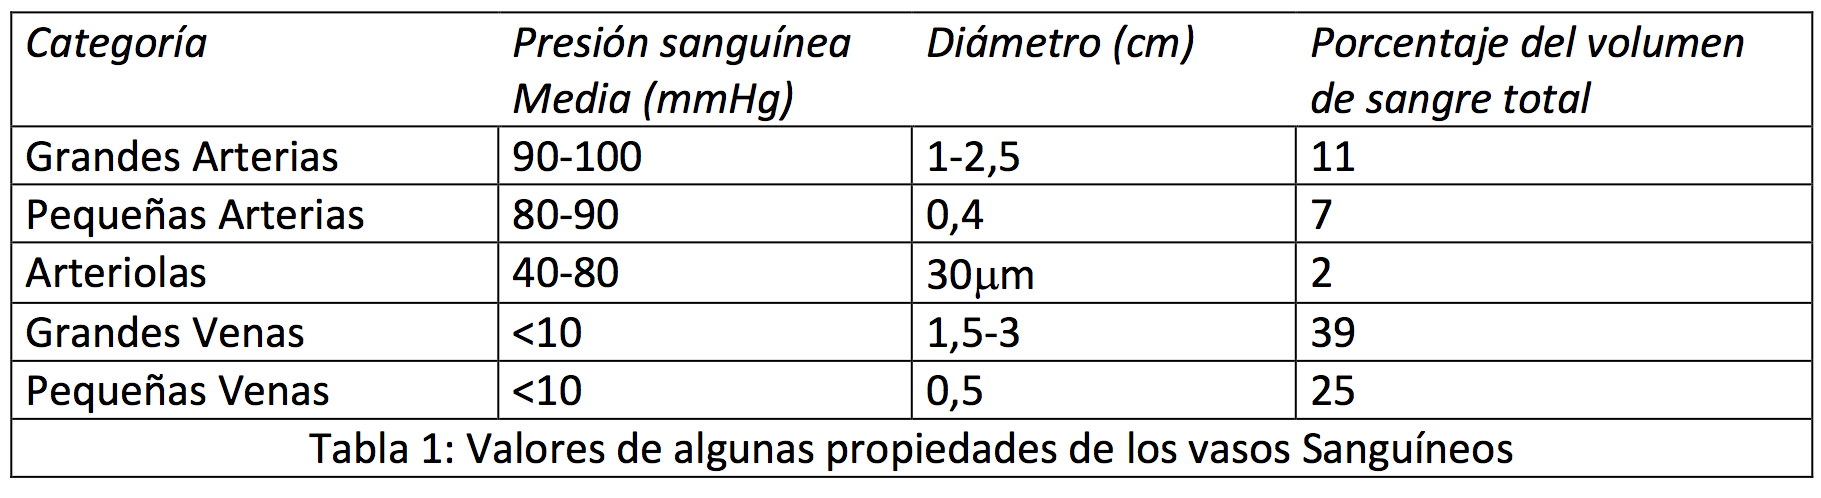
\includegraphics[width=0.75\textwidth]{table-1}
			\end{center}
		\end{figure}

		\begin{figure}[H]
			\begin{center}
				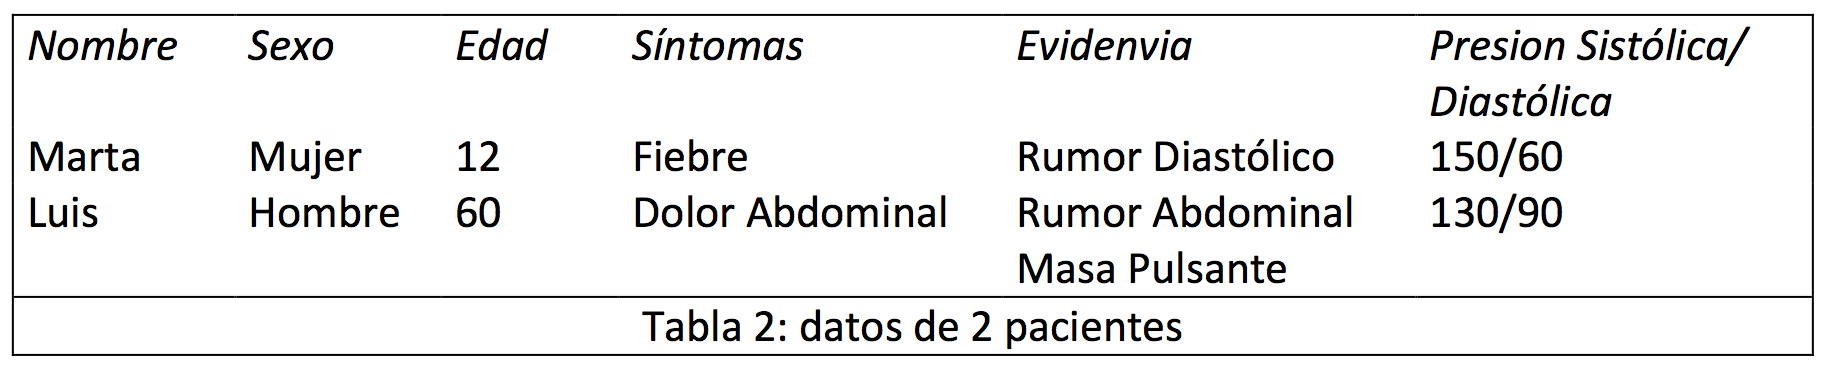
\includegraphics[width=0.75\textwidth]{table-2}
			\end{center}
		\end{figure}

		\paragraph{}
		La base de conocimiento necesaria para representar el problema requiere de un conjunto tanto de objetos como de atributos de los mismos. Esto se describe a continuación a partir de la Definición del Dominio (DD) y el conjunto de reglas:

		\begin{equation*}
			O = \{paciente, enfermedad, queja, riesgo \}
		\end{equation*}

		\begin{multline*}
			DA = \{ \\
				enfermedad.tipo^s, enfermedad.subtipo^s, enfermedad.lugar^s, \\
				paciente.edad^s:number, paciente.queja^m, \\
				paciente.sistolica^s:number, paciente.sistolica^s:number, paciente.pulso^s:number, \\
				paciente.auscultacion^m, paciente.riesgo^m \\
				queja.nombre^s, queja.duracion^s:number, queja.lugar^s\\
				riesgo.nombre^s, riesgo.duraccion^s:number\\
			\}
		\end{multline*}


		\begin{enumerate}[label={\textbf{R\theenumi:}}]

			\item
				\textbf{if} $equals(combustibleEnMotor, estado, f)$ \textbf{and} $equals(depositoCombustible, observacion, cero)$ \\
				\textbf{then} $add(depositoCombustible, estado, vacio)$ \textbf{fi}

		\end{enumerate}

\end{document}
